% Template:     Informe LaTeX
% Documento:    Archivo de ejemplo
% Versión:      8.1.7 (24/07/2022)
% Codificación: UTF-8
%
% Autor: Pablo Pizarro R.
%        pablo@ppizarror.com
%
% Manual template: [https://latex.ppizarror.com/informe]
% Licencia MIT:    [https://opensource.org/licenses/MIT]

\section{Definición del Problema}

Desde la declaración de la pandemia Covid19 a nivel mundial, muchos han sido los esfuerzos de realizar acciones para entender y controlar el desarrollo de esta pandemia, sin embargo desde el campo de computación han surgido la necesidad de establecer herramientas que permitan análisis visual \scite{alsakran2020visual} que incorporen varios diseños visuales y análisis de las tendencias de propagación, con el objetivo de promover la comprensión de como se comportan los datos, ahora bien, a pesar que la pandemia a terminado, consideramos que sigue siendo una necesidad para el gobierno peruano y las instituciones llamadas a contribuir con herramientas que permitan el análisis y visualización de datos con otras enfermedades que azota al país como el caso del dengue, razón por la cual abordamos el presente trabajo.


\section{Descripción de la Base de Datos}


Covid19Mexico.csv \scite{salud} es una base de datos abiertos gestionado por la dirección general de epidemiología de la secretaría de salud de México, Conforme al Decreto publicado en el diario Oficial de la Federación el 20 de Febrero del 2015, que establece la regulación en materia de Datos Abiertos, la Dirección General de Epidemiología, con base en los ordenamientos aplicables en dicha materia, pone a disposición de la población en general, la información contenida en los Anuarios Estadísticos de Morbilidad 2015-2017, así como la información referente a los casos asociados a COVID-19 \scite{klein2023spatial} con el propósito de facilitar a todos los usuarios que la requieran, el acceso, uso, reutilización y redistribución de la misma.


\subsection{Definición de cada Atributo}
El \textit{dataset} fue obtenido del sitio web de datos abiertos del gobierno de los Estados Unidos Mexicanos \scite{Salud}, donde podemos encontrar toda la data
recolectada desde el 27 de noviembre de 2020 hasta el 16 de mayo de 2023; sin embargo, para este caso  tomaremos la base de datos que cuenta con 7294030 registros. Se escogió data, ya que permite ya que es mas manejable el análisis estadístico descriptivo y posibilitar su ejecución en computadores con características normales. En base al dataset recolectado se tienen los siguientes atributos:

\begin{enumerate}
	\item \textbf{FECHA\_ACTUALIZACION}: La base de datos se alimenta diariamente, esta variable permite identificar la fecha de la ultima actualizacion. AAAA-MM-DD
	\item \textbf{ID\_REGISTRO}: Número identificador del caso, TEXTO
	\item \textbf{ORIGEN}: La vigilancia centinela se realiza a través del sistema de unidades de salud monitoras de enfermedades respiratorias (USMER). Las USMER incluyen unidades médicas del primer, segundo o tercer nivel de atención y también participan como USMER las unidades de tercer nivel que por sus características contribuyen a ampliar el panorama de información epidemiológica, entre ellas las que cuenten con especialidad de neumología, infectología o pediatría. (Categorías en Catalógo Anexo). CATÁLOGO: ORIGEN
	\item \textbf{SECTOR}: Identifica el tipo de institución del Sistema Nacional de Salud que brindó la atención. CATÁLOGO: SECTOR
	\item \textbf{ENTIDAD\_UM}: Identifica la entidad donde se ubica la unidad medica que brindó la atención. CATALÓGO: ENTIDADES
	\item \textbf{SEXO}: Identifica al sexo del paciente. CATÁLOGO: SEXO
	\item \textbf{ENTIDAD\_NAC}: Identifica la entidad de nacimiento del paciente. CATALÓGO: ENTIDADES
	\item \textbf{ENTIDAD\_RES}: Identifica la entidad de residencia del paciente. CATALÓGO: ENTIDADES
	\item \textbf{MUNICIPIO\_RES}: Identifica el municipio de residencia del paciente. CATALÓGO: MUNICIPIOS
	\item \textbf{TIPO\_PACIENTE}: Identifica el tipo de atención que recibió el paciente en la unidad. Se denomina como ambulatorio si regresó a su casa o se denomina como hospitalizado si fue ingresado a hospitalización. CATÁLOGO: TIPO\_PACIENTE
	\item \textbf{FECHA\_INGRESO}: Identifica la fecha de ingreso del paciente a la unidad de atención. AAAA-MM-DD
	\item \textbf{FECHA\_SINTOMAS}: Idenitifica la fecha en que inició la sintomatología del paciente. AAAA-MM-DD
	\item \textbf{FECHA\_DEF}: Identifica la fecha en que el paciente falleció. AAAA-MM-DD
	\item \textbf{INTUBADO}: Identifica si el paciente requirió de intubación. CATÁLOGO: SI\_NO
	\item \textbf{NEUMONIA}: Identifica si al paciente se le diagnosticó con neumonía. CATÁLOGO: SI\_NO
	\item \textbf{EDAD}: Identifica la edad del paciente. NÚMERICA EN AÑOS
	\item \textbf{NACIONALIDAD}: Identifica si el paciente es mexicano o extranjero. CATÁLOGO: NACIONALIDAD
	\item \textbf{EMBARAZO}: Identifica si la paciente está embarazada. CATÁLOGO: SI\_NO
	\item \textbf{HABLA\_LENGUA\_INDIG}: Identifica si el paciente habla lengua índigena. CATÁLOGO: SI\_NO
	\item \textbf{INDIGENA}: Identifica si el paciente se autoidentifica como una persona indígena. CATÁLOGO: SI\_NO
	\item \textbf{DIABETES}: Identifica si el paciente tiene un diagnóstico de diabetes. CATÁLOGO: SI\_NO
	\item \textbf{EPOC}: Identifica si el paciente tiene un diagnóstico de EPOC. CATÁLOGO: SI\_NO
	\item \textbf{ASMA}: Identifica si el paciente tiene un diagnóstico de asma. CATÁLOGO: SI\_NO
	\item \textbf{INMUSUPR}: Identifica si el paciente presenta inmunosupresión. CATÁLOGO: SI\_NO
	\item \textbf{HIPERTENSION}: Identifica si el paciente tiene un diagnóstico de hipertensión. CATÁLOGO: SI\_NO
	\item \textbf{OTRA\_COM}: Identifica si el paciente tiene diagnóstico de otras enfermedades. CATÁLOGO: SI\_NO
	\item \textbf{CARDIOVASCULAR}: Identifica si el paciente tiene un diagnóstico de enfermedades cardiovasculares. CATÁLOGO: SI\_NO
	\item \textbf{OBESIDAD}: Identifica si el paciente tiene diagnóstico de obesidad. CATÁLOGO: SI\_NO
	\item \textbf{RENAL\_CRONICA}: Identifica si el paciente tiene diagnóstico de insuficiencia renal crónica. CATÁLOGO: SI\_NO
	\item \textbf{TABAQUISMO}: Identifica si el paciente tiene hábito de tabaquismo. CATÁLOGO: SI\_NO
	\item \textbf{OTRO\_CASO}: Identifica si el paciente tuvo contacto con algún otro caso diagnósticado con SARS CoV-2. CATÁLOGO: SI\_NO
	\item \textbf{TOMA\_MUESTRA\_LAB}: Identifica si al paciente se le tomó muestra de laboratorio. CATÁLOGO: SI\_NO
	\item \textbf{RESULTADO\_LAB}: Identifica el resultado del análisis de la muestra reportado por el  laboratorio de la Red Nacional de Laboratorios de Vigilancia Epidemiológica (INDRE, LESP y LAVE) y laboratorios privados avalados por el InDRE cuyos resultados son registrados en SISVER. (Catálogo de resultados diagnósticos anexo). CATÁLOGO: RESULTADO\_LAB
	\item \textbf{TOMA\_MUESTRA\_ANTIGENO}: Identifica si al paciente se le tomó muestra de antígeno para SARS-CoV-2. CATÁLOGO: SI\_NO
	\item \textbf{RESULTADO\_ANTIGENO}: Identifica el resultado del análisis de la muestra de antígeno tomada al paciente. CATÁLOGO: RESULTADO\_ANTIGENO
	\item \textbf{CLASIFICACION\_FINAL}: Identifica si el paciente es un caso de COVID\-19 según el catálogo ``CLASIFICACION\_FINAL''. CATÁLOGO: CLASIFICACION\_FINAL
	\item \textbf{MIGRANTE}: Identifica si el paciente es una persona migrante. CATÁLOGO: SI\_NO
	\item \textbf{PAIS\_NACIONALIDAD}: Identifica la nacionalidad del paciente. TEXTO, 99\=SE IGNORA
	\item \textbf{PAIS\_ORIGEN}: Identifica el país del que partió el paciente rumbo a México. TEXTO, 97\=NO APLICA
	\item \textbf{UCI}: Identifica si el paciente requirió ingresar a una Unidad de Cuidados Intensivos. CATÁLOGO: SI\_NO
\end{enumerate}

\clearpage

\subsection{Distribución de las Variables}
\subsubsection{Tipos de Datos de las columnas del \emph{dataset}}
En la \ref{tabla:datatype} se puede apreciar los tipos de dato para cada columna del \emph{dataset}. Se puede apreciar que las fechas se detectan como \emph{object}, por lo cual será necesario hacer una transformación de dichos datos.

\begin{table}[h]
\resizebox{7.5cm}{!} {

\begin{tabular}{|l|l|l|}
\hline
\# & Variable                & T. de dato \\ \hline
1  & FECHA\_ACTUALIZACION    & object     \\ \hline
2  & ID\_REGISTRO            & object     \\ \hline
3  & ORIGEN                  & int64      \\ \hline
4  & SECTOR                  & int64      \\ \hline
5  & ENTIDAD\_UM             & int64      \\ \hline
6  & SEXO                    & int64      \\ \hline
7  & ENTIDAD\_NAC            & int64      \\ \hline
8  & ENTIDAD\_RES            & int64      \\ \hline
9  & MUNICIPIO\_RES          & int64      \\ \hline
10 & TIPO\_PACIENTE          & int64      \\ \hline
11 & FECHA\_INGRESO          & object     \\ \hline
12 & FECHA\_SINTOMAS         & object     \\ \hline
13 & FECHA\_DEF              & object     \\ \hline
14 & INTUBADO                & int64      \\ \hline
15 & NEUMONIA                & int64      \\ \hline
16 & EDAD                    & int64      \\ \hline
17 & NACIONALIDAD            & int64      \\ \hline
18 & EMBARAZO                & int64      \\ \hline
19 & HABLA\_LENGUA\_INDIG    & int64      \\ \hline
20 & INDIGENA                & int64      \\ \hline
21 & DIABETES                & int64      \\ \hline
22 & EPOC                    & int64      \\ \hline
23 & ASMA                    & int64      \\ \hline
24 & INMUSUPR                & int64      \\ \hline
25 & HIPERTENSION            & int64      \\ \hline
26 & OTRA\_COM               & int64      \\ \hline
27 & CARDIOVASCULAR          & int64      \\ \hline
28 & OBESIDAD                & int64      \\ \hline
29 & RENAL\_CRONICA          & int64      \\ \hline
30 & TABAQUISMO              & int64      \\ \hline
31 & OTRO\_CASO              & int64      \\ \hline
32 & TOMA\_MUESTRA\_LAB      & int64      \\ \hline
33 & RESULTADO\_LAB          & int64      \\ \hline
34 & TOMA\_MUESTRA\_ANTIGENO & int64      \\ \hline
35 & RESULTADO\_ANTIGENO     & int64      \\ \hline
36 & CLASIFICACION\_FINAL    & int64      \\ \hline
37 & MIGRANTE                & int64      \\ \hline
38 & PAIS\_NACIONALIDAD      & object     \\ \hline
39 & PAIS\_ORIGEN            & object     \\ \hline
40 & UCI                     & int64      \\ \hline
\end{tabular}
}
\caption{Tipos de datos del \emph{dataset}.}
\label{tabla:datatype}
\end{table}

\clearpage
\subsubsection{Valores no Nulos y Valores Nulos}
\begin{table}[h]
\resizebox{10cm}{!} {
\begin{tabular}{|l|l|c|c|}
\hline
\# & Variable & \multicolumn{1}{l|}{\# Valores Nulos} & \multicolumn{1}{l|}{\# Valores no Nulos} \\ \hline
1  & FECHA\_ACTUALIZACION    & 0 & 7294030 \\ \hline
2  & ID\_REGISTRO            & 0 & 7294030 \\ \hline
3  & ORIGEN                  & 0 & 7294030 \\ \hline
4  & SECTOR                  & 0 & 7294030 \\ \hline
5  & ENTIDAD\_UM             & 0 & 7294030 \\ \hline
6  & SEXO                    & 0 & 7294030 \\ \hline
7  & ENTIDAD\_NAC            & 0 & 7294030 \\ \hline
8  & ENTIDAD\_RES            & 0 & 7294030 \\ \hline
9  & MUNICIPIO\_RES          & 0 & 7294030 \\ \hline
10 & TIPO\_PACIENTE          & 0 & 7294030 \\ \hline
11 & FECHA\_INGRESO          & 0 & 7294030 \\ \hline
12 & FECHA\_SINTOMAS         & 0 & 7294030 \\ \hline
13 & FECHA\_DEF              & 0 & 7294030 \\ \hline
14 & INTUBADO                & 0 & 7294030 \\ \hline
15 & NEUMONIA                & 0 & 7294030 \\ \hline
16 & EDAD                    & 0 & 7294030 \\ \hline
17 & NACIONALIDAD            & 0 & 7294030 \\ \hline
18 & EMBARAZO                & 0 & 7294030 \\ \hline
19 & HABLA\_LENGUA\_INDIG    & 0 & 7294030 \\ \hline
20 & INDIGENA                & 0 & 7294030 \\ \hline
21 & DIABETES                & 0 & 7294030 \\ \hline
22 & EPOC                    & 0 & 7294030 \\ \hline
23 & ASMA                    & 0 & 7294030 \\ \hline
24 & INMUSUPR                & 0 & 7294030 \\ \hline
25 & HIPERTENSION            & 0 & 7294030 \\ \hline
26 & OTRA\_COM               & 0 & 7294030 \\ \hline
27 & CARDIOVASCULAR          & 0 & 7294030 \\ \hline
28 & OBESIDAD                & 0 & 7294030 \\ \hline
29 & RENAL\_CRONICA          & 0 & 7294030 \\ \hline
30 & TABAQUISMO              & 0 & 7294030 \\ \hline
31 & OTRO\_CASO              & 0 & 7294030 \\ \hline
32 & TOMA\_MUESTRA\_LAB      & 0 & 7294030 \\ \hline
33 & RESULTADO\_LAB          & 0 & 7294030 \\ \hline
34 & TOMA\_MUESTRA\_ANTIGENO & 0 & 7294030 \\ \hline
35 & RESULTADO\_ANTIGENO     & 0 & 7294030 \\ \hline
36 & CLASIFICACION\_FINAL    & 0 & 7294030 \\ \hline
37 & MIGRANTE                & 0 & 7294030 \\ \hline
38 & PAIS\_NACIONALIDAD      & 0 & 7294030 \\ \hline
39 & PAIS\_ORIGEN            & 0 & 7294030 \\ \hline
40 & UCI                     & 0 & 7294030 \\ \hline
\end{tabular}
}
\caption{Valores nulos y no nulos encontrados en el dataset.}
\label{tabla:autores}
\end{table}

\clearpage
\subsubsection{Valores únicos}

\begin{table}[h]
\resizebox{7cm}{!} {
\begin{tabular}{|l|c|}
\hline
FECHA\_ACTUALIZACION    & 1                        \\ \hline
ID\_REGISTRO            & 7294030                  \\ \hline
ORIGEN                  & 2                        \\ \hline
SECTOR                  & 14                       \\ \hline
ENTIDAD\_UM             & 32                       \\ \hline
SEXO                    & 2                        \\ \hline
ENTIDAD\_NAC            & 33                       \\ \hline
ENTIDAD\_RES            & 32                       \\ \hline
MUNICIPIO\_RES          & 550                      \\ \hline
TIPO\_PACIENTE          & 2                        \\ \hline
FECHA\_INGRESO          & 501                      \\ \hline
FECHA\_SINTOMAS         & 501                      \\ \hline
FECHA\_DEF              & 501                      \\ \hline
INTUBADO                & 4                        \\ \hline
NEUMONIA                & 3                        \\ \hline
EDAD                    & 131                      \\ \hline
NACIONALIDAD            & 2                        \\ \hline
EMBARAZO                & 5                        \\ \hline
HABLA\_LENGUA\_INDIG    & 3                        \\ \hline
INDIGENA                & 3                        \\ \hline
DIABETES                & 3                        \\ \hline
EPOC                    & 3                        \\ \hline
ASMA                    & 3                        \\ \hline
INMUSUPR                & 3                        \\ \hline
HIPERTENSION            & 3                        \\ \hline
OTRA\_COM               & 3                        \\ \hline
CARDIOVASCULAR          & 3                        \\ \hline
OBESIDAD                & 3                        \\ \hline
RENAL\_CRONICA          & 3                        \\ \hline
TABAQUISMO              & 3                        \\ \hline
OTRO\_CASO              & 3                        \\ \hline
TOMA\_MUESTRA\_LAB      & 2                        \\ \hline
RESULTADO\_LAB          & 5                        \\ \hline
TOMA\_MUESTRA\_ANTIGENO & \multicolumn{1}{l|}{2}   \\ \hline
RESULTADO\_ANTIGENO     & \multicolumn{1}{l|}{3}   \\ \hline
CLASIFICACION\_FINAL    & \multicolumn{1}{l|}{7}   \\ \hline
MIGRANTE                & \multicolumn{1}{l|}{3}   \\ \hline
PAIS\_NACIONALIDAD      & \multicolumn{1}{l|}{177} \\ \hline
PAIS\_ORIGEN            & \multicolumn{1}{l|}{113} \\ \hline
UCI                     & \multicolumn{1}{l|}{4}   \\ \hline
\end{tabular}
}
\caption{Cantidad de valores únicos.}
\label{tabla:autores}
\end{table}

\textbf{Valores únicos por columna}
\begin{lstlisting}[language=haskell, caption=Valores por columna, captionpos=b, label=lst:fiboHaskell]

FECHA_ACTUALIZACION
['2023-05-16']

ID_REGISTRO
['0741e4' '0ed066' '08c5f9' ... 'm19f073' 'm1e288e' 'm1029da']

ORIGEN
[2 1]

SECTOR
[ 6 12  3  9 10 11  8  7  1  4  5 13  2 99]

ENTIDAD_UM
[ 9 16 15 12 22 18 20 14 23 25  3 10  7 17 24  5  1 21 28 26 27 19  4  2
 32 31  8 13 11 30  6 29]

SEXO
[2 1]

ENTIDAD_NAC
[ 9 16 12 18 20 32  8 25 14 10  7 27  6 13 15 17 22 24  5 21 28 26 19  2
 31  1  3 11 29 30 99  4 23]

ENTIDAD_RES
[ 9 16 15 12 22 18 20 14 23 25  3 10  7 17 24  5  1 21 28 26 27 19  4  2
 32 31  8 13 11 30  6 29]

MUNICIPIO_RES
[ 16  41  60   2  14  29  15   7  67  71   6   8   1  12  10   3   5  59
  35   4  33  19  28  49  76  30  53   9  46  13  22  17  58  56  32  50
  37  18 515  57  25  66 120  77 413 109 104  42  62  26  89 324  20 375
  34  21 101  11 114  65 155 193 184  52  31  78 122  70  24 156  68  43
  40 102 112  55 115  38  88 108 121  48  39 119 111 177  86  97  23 134
  64  99  27 106  79  45  44 417  87  51 338  95  81  63  36 138  93 118
  83 174  98  69 157 208 133 105  54 140 100 103  94 385 483 164  75 107
 113  82 379  74  85  96 207 327 163 397 178 183 204 132 189 110  91 294
 293 187 390  47 211  90 175 137 530 131 124 116 318  92 482 232 227 141
 170 154 234 169 126 551 565  84 201 172 505  61 186 399 166 462 350 145
 561 150 364  73 564 191 181 143 196 206  80 190 277 330 135 123 127 295
 310 214 403 570  72 160 161 153 152 162 200 314 539 519 469 497 125 130
 149 148 418 128 192 197 266 180 557 268 525 182 342 315 459 247 265 147
 203 420 199 298 545 205 552 553 129 544 212 401 179 188 358 185 476 348
 521 117 194 447 171 409 550 325 509 198 396 440 345 400 176 173 168 243
 139 301 144 307 217 213 210 337 209 387 398 142 278 508 546 279 146 369
 360 317 230 414 136 159 427 432 467 380 334 280 439 231 356 455 252 559
 453 248 465 305 151 229 272 513 426 549 195 431 999 555 333 158 526 165
 512 456 560 343 275 543 253 568 306 415 421 260 300 499 349 202 475 291
 378 452 516 407 480 520 368 308 391 498 215 288 393 540 429 344 384 441
 458 406 235 517 558 216 533 363 472 347 419 386 249 237 351 372 537 502
 167 531 466 286 495 446 239 312 267 529 454 468 238 449 289 554 259 309
 567 296 412 225 362 388 366 254 381 303 411 496 242 367 486 487 534 450
 302 504 510 339 425 370 410 261 244 273 424 485 474 224 528 285 494 365
 511 353 527 500 271 442 542 569 523 269 547 477 383 263 359 514 371 292
 240 444 251 219 503 473 541 438 392 405 245 336 373 377 402 332 448 463
 478 326 493 233 522 404 491 562 507 241 490 460 250 341 443 395 423 437
 457 538 389 284 329 270 416 492 297 435 346 535 281 355 374 445 257 470
 255 323 408 246 524 422 287 394 222 489 566 352 319 221 264 316 283 436
 304 536 290 226 321 335 313 434 471 461 340 428 274 311 354 258 548 563
 220 501 532 484 276 481 299 556 433 506]

TIPO_PACIENTE
[2 1]

FECHA_INGRESO
['2022-02-20' '2023-03-09' '2022-01-11' '2022-08-07' '2022-05-22'
 '2022-01-20' '2022-02-18' '2022-02-08' '2022-06-23' '2022-08-09'
 '2022-01-12' '2022-07-22' '2022-08-24' '2022-02-14' '2022-01-19'
 '2022-05-03' '2022-01-17' '2022-07-26' '2022-03-05' '2022-03-09'
 '2022-08-23' '2022-03-07' '2022-08-02' '2022-03-06' '2022-01-05'
 '2022-02-16' '2022-01-28' '2022-01-15' '2022-07-21' '2022-08-30'
 '2022-07-07' '2022-12-23' '2022-01-01' '2022-06-14' '2022-07-20'
 '2022-06-28' '2022-06-20' '2022-06-16' '2022-06-29' '2022-05-19'
 '2022-04-26' '2022-07-28' '2022-10-23' '2022-12-18' '2022-01-09'
 '2022-07-14' '2022-08-18' '2022-12-05' '2022-04-11' '2022-07-06'
 '2022-01-13' '2022-02-02' '2023-04-26' '2022-09-07' '2022-03-20'
 '2022-01-26' '2022-06-25' '2022-01-24' '2022-07-17' '2023-03-02'
 '2022-06-19' '2023-04-04' '2022-01-10' '2022-08-03' '2022-08-19'
 '2022-02-01' '2022-02-21' '2022-12-19' '2022-09-05' '2022-01-06'
 '2022-12-16' '2022-06-24' '2022-01-31' '2023-02-03' '2023-01-01'
 '2022-01-30' '2022-07-12' '2022-01-04' '2023-03-20' '2022-01-22'
 '2022-01-03' '2022-05-11' '2022-02-17' '2022-01-08' '2022-09-27'
 '2022-01-29' '2022-10-13' '2022-03-14' '2022-09-06' '2022-07-25'
 '2022-01-21' '2022-03-24' '2022-01-16' '2022-02-24' '2022-06-22'
 '2022-09-30' '2022-07-05' '2022-06-08' '2022-02-10' '2023-02-20'
 '2022-01-14' '2022-11-19' '2022-01-07' '2022-06-06' '2023-02-07'
 '2023-02-15' '2022-02-15' '2022-02-03' '2023-01-15' '2022-01-25'
 '2023-02-24' '2023-02-28' '2023-03-01' '2022-01-18' '2022-02-11'
 '2022-07-15' '2022-03-13' '2022-07-10' '2022-03-12' '2022-04-18'
 '2023-03-24' '2022-08-15' '2023-03-07' '2022-02-23' '2022-03-26'
 '2023-03-06' '2022-09-09' '2022-06-30' '2023-02-26' '2022-01-23'
 '2022-07-18' '2022-03-16' '2022-07-13' '2022-10-22' '2022-03-03'
 '2022-02-22' '2022-02-28' '2022-06-27' '2022-07-19' '2022-03-01'
 '2022-07-08' '2022-04-04' '2022-06-13' '2022-05-12' '2023-03-28'
 '2022-07-01' '2022-07-24' '2022-03-30' '2022-12-12' '2023-01-19'
 '2022-12-17' '2023-04-15' '2023-03-04' '2022-09-10' '2022-03-11'
 '2022-07-27' '2022-12-14' '2022-11-14' '2022-01-27' '2022-03-04'
 '2022-12-29' '2022-03-02' '2022-03-08' '2022-05-18' '2023-01-04'
 '2022-06-10' '2022-03-22' '2022-08-01' '2022-07-11' '2022-11-24'
 '2023-01-07' '2022-04-13' '2022-03-19' '2022-07-29' '2022-09-29'
 '2022-12-11' '2022-02-04' '2022-05-20' '2022-06-26' '2022-02-09'
 '2022-09-15' '2022-02-25' '2022-07-04' '2022-05-24' '2022-02-13'
 '2022-08-06' '2022-03-17' '2022-07-16' '2022-01-02' '2023-03-14'
 '2022-09-23' '2022-05-13' '2022-12-09' '2022-03-28' '2022-08-10'
 '2022-02-06' '2022-06-18' '2022-12-10' '2023-05-05' '2023-02-27'
 '2022-08-16' '2022-07-09' '2023-05-06' '2022-09-28' '2023-01-27'
 '2022-03-23' '2023-01-20' '2022-03-18' '2022-08-26' '2023-03-25'
 '2022-03-29' '2022-05-29' '2022-05-30' '2022-02-05' '2022-04-06'
 '2022-03-15' '2022-05-16' '2022-08-12' '2022-04-20' '2022-05-27'
 '2022-10-01' '2022-03-27' '2022-06-17' '2022-08-29' '2022-08-22'
 '2022-10-06' '2022-07-23' '2022-12-13' '2022-11-28' '2023-01-12'
 '2022-02-26' '2022-04-17' '2022-05-02' '2022-02-27' '2022-08-20'
 '2022-09-19' '2023-01-30' '2022-11-09' '2022-05-23' '2022-03-25'
 '2022-02-19' '2022-10-07' '2022-04-07' '2022-04-01' '2022-12-06'
 '2023-01-09' '2022-04-10' '2022-04-09' '2022-03-21' '2022-10-05'
 '2022-04-05' '2022-04-02' '2022-04-08' '2022-03-31' '2023-01-02'
 '2022-10-11' '2022-12-20' '2022-04-19' '2022-04-15' '2023-01-11'
 '2022-04-14' '2022-04-12' '2022-12-01' '2023-03-21' '2022-03-10'
 '2022-05-10' '2023-02-14' '2022-06-15' '2022-04-03' '2022-07-31'
 '2022-02-07' '2022-09-26' '2022-02-12' '2023-01-31' '2022-11-18'
 '2023-01-14' '2022-08-31' '2022-08-08' '2022-11-29' '2022-11-01'
 '2023-01-13' '2023-01-23' '2022-12-26' '2022-05-14' '2022-06-12'
 '2022-12-28' '2022-06-04' '2022-06-21' '2023-01-16' '2022-12-04'
 '2023-03-31' '2023-02-22' '2022-06-05' '2022-11-08' '2022-04-16'
 '2022-08-25' '2022-12-22' '2023-02-21' '2022-08-17' '2022-05-25'
 '2022-09-14' '2023-01-18' '2022-09-20' '2022-12-15' '2023-04-18'
 '2022-10-12' '2022-07-03' '2023-01-05' '2023-01-17' '2023-04-19'
 '2022-11-23' '2022-07-30' '2022-10-15' '2022-11-04' '2022-04-21'
 '2022-09-12' '2022-08-11' '2022-06-09' '2022-10-10' '2022-04-30'
 '2022-12-30' '2022-04-22' '2023-04-03' '2022-04-24' '2022-04-23'
 '2022-06-07' '2022-05-08' '2022-04-28' '2022-04-29' '2022-05-01'
 '2022-06-11' '2022-04-25' '2022-04-27' '2022-12-03' '2022-05-28'
 '2022-12-24' '2022-05-26' '2022-05-04' '2022-05-06' '2022-05-05'
 '2022-05-07' '2022-05-15' '2022-09-11' '2022-05-09' '2022-10-21'
 '2022-11-10' '2022-05-17' '2022-05-21' '2022-05-31' '2022-09-01'
 '2022-06-02' '2022-06-01' '2022-06-03' '2022-10-09' '2022-09-21'
 '2022-10-26' '2022-07-02' '2022-09-04' '2023-03-27' '2022-12-21'
 '2023-03-30' '2023-02-10' '2022-09-08' '2022-11-22' '2022-11-25'
 '2022-09-13' '2022-09-22' '2022-10-24' '2022-11-15' '2022-08-04'
 '2022-08-28' '2022-08-05' '2022-12-02' '2022-09-02' '2023-01-25'
 '2023-05-02' '2022-08-14' '2022-08-13' '2022-08-21' '2022-08-27'
 '2022-09-03' '2022-09-16' '2023-03-22' '2023-03-17' '2022-10-08'
 '2022-10-18' '2022-09-18' '2022-10-20' '2022-09-24' '2022-09-17'
 '2022-10-16' '2022-12-07' '2022-09-25' '2022-12-31' '2022-10-04'
 '2022-10-03' '2022-10-02' '2022-11-30' '2022-10-19' '2022-10-28'
 '2022-10-25' '2022-11-11' '2022-10-14' '2023-03-12' '2022-10-17'
 '2022-11-16' '2022-10-27' '2022-12-08' '2022-10-29' '2022-10-30'
 '2023-02-19' '2022-10-31' '2022-11-03' '2022-11-02' '2022-11-07'
 '2022-11-05' '2022-11-06' '2023-01-06' '2022-11-12' '2022-11-13'
 '2022-11-17' '2022-11-21' '2022-11-20' '2022-11-26' '2022-12-27'
 '2022-11-27' '2022-12-25' '2023-01-03' '2023-01-10' '2023-02-16'
 '2023-02-17' '2023-01-24' '2023-04-17' '2023-01-08' '2023-04-20'
 '2023-02-13' '2023-03-23' '2023-01-22' '2023-01-21' '2023-01-29'
 '2023-02-23' '2023-02-02' '2023-04-09' '2023-01-28' '2023-01-26'
 '2023-02-01' '2023-02-06' '2023-02-09' '2023-04-24' '2023-02-04'
 '2023-02-25' '2023-02-05' '2023-02-08' '2023-02-18' '2023-02-11'
 '2023-02-12' '2023-03-03' '2023-03-16' '2023-03-08' '2023-03-11'
 '2023-03-05' '2023-03-13' '2023-03-10' '2023-03-15' '2023-03-18'
 '2023-03-19' '2023-03-26' '2023-03-29' '2023-04-05' '2023-04-06'
 '2023-04-02' '2023-04-01' '2023-05-09' '2023-04-08' '2023-04-11'
 '2023-04-07' '2023-04-10' '2023-04-12' '2023-05-01' '2023-04-13'
 '2023-04-14' '2023-04-16' '2023-04-23' '2023-04-25' '2023-04-21'
 '2023-04-22' '2023-05-11' '2023-04-28' '2023-04-27' '2023-05-04'
 '2023-04-29' '2023-04-30' '2023-05-12' '2023-05-03' '2023-05-10'
 '2023-05-08' '2023-05-07' '2023-05-14' '2023-05-13' '2023-05-15'
 '2023-05-16']

FECHA_SINTOMAS
['2022-02-13' '2023-03-06' '2022-01-09' '2022-02-20' '2022-08-07'
 '2022-05-22' '2022-01-16' '2022-02-18' '2022-02-05' '2022-06-21'
 '2022-08-06' '2022-01-12' '2022-07-20' '2022-08-22' '2022-02-14'
 '2022-01-17' '2022-05-03' '2022-07-26' '2022-03-05' '2022-03-09'
 '2022-08-21' '2022-03-07' '2022-07-31' '2022-03-03' '2022-03-06'
 '2022-01-01' '2022-02-16' '2022-01-24' '2022-01-15' '2022-08-30'
 '2022-07-01' '2022-01-08' '2022-07-14' '2022-12-23' '2022-06-09'
 '2022-07-15' '2022-06-28' '2022-06-17' '2022-06-13' '2022-05-19'
 '2022-04-22' '2022-07-25' '2022-10-10' '2022-12-12' '2022-07-12'
 '2022-08-17' '2022-12-04' '2022-04-09' '2022-01-10' '2022-02-06'
 '2022-02-02' '2023-04-22' '2022-09-04' '2022-03-15' '2022-01-23'
 '2022-06-23' '2022-07-13' '2022-01-22' '2023-03-01' '2022-07-03'
 '2022-06-18' '2023-04-04' '2022-01-06' '2022-08-02' '2022-08-14'
 '2022-01-31' '2022-07-02' '2022-07-07' '2022-01-19' '2022-12-18'
 '2022-01-02' '2022-12-16' '2022-06-26' '2022-06-24' '2022-01-28'
 '2022-01-03' '2023-02-03' '2022-12-30' '2022-01-05' '2022-01-27'
 '2022-07-10' '2023-03-16' '2022-01-20' '2022-12-01' '2022-05-10'
 '2022-01-18' '2022-01-07' '2022-09-23' '2022-01-14' '2022-10-07'
 '2022-01-04' '2022-04-26' '2022-09-01' '2022-09-05' '2022-09-03'
 '2022-01-25' '2022-03-22' '2022-06-22' '2022-02-24' '2022-09-28'
 '2022-05-25' '2022-02-09' '2023-02-18' '2022-06-25' '2022-01-11'
 '2022-11-15' '2022-06-29' '2022-06-05' '2023-02-07' '2022-01-26'
 '2022-01-13' '2023-02-15' '2022-02-15' '2022-02-01' '2023-01-15'
 '2022-01-30' '2022-07-04' '2022-02-17' '2022-08-01' '2023-02-20'
 '2022-05-04' '2023-02-25' '2022-05-02' '2023-02-26' '2022-07-21'
 '2022-02-11' '2022-01-21' '2022-07-09' '2022-03-12' '2022-04-16'
 '2023-03-19' '2022-02-03' '2022-08-11' '2023-03-04' '2022-08-15'
 '2022-05-31' '2022-02-19' '2022-03-26' '2023-03-05' '2022-06-27'
 '2023-02-22' '2022-02-10' '2022-07-11' '2022-07-08' '2023-02-27'
 '2022-01-29' '2022-10-19' '2022-02-28' '2022-02-08' '2022-07-17'
 '2022-02-27' '2023-01-01' '2022-07-24' '2022-12-19' '2022-04-02'
 '2022-06-12' '2022-05-12' '2023-03-24' '2022-03-27' '2022-12-10'
 '2022-06-20' '2023-01-14' '2022-12-15' '2023-04-15' '2022-03-11'
 '2022-07-19' '2022-11-11' '2022-03-04' '2022-12-28' '2022-08-03'
 '2022-03-14' '2022-03-02' '2022-03-08' '2022-05-17' '2022-07-22'
 '2022-07-29' '2022-12-31' '2022-06-10' '2022-03-21' '2022-07-27'
 '2022-03-29' '2022-11-19' '2022-07-05' '2023-01-06' '2022-04-12'
 '2022-09-26' '2022-12-09' '2022-04-04' '2022-07-06' '2022-09-15'
 '2022-03-24' '2022-02-25' '2022-05-24' '2022-02-04' '2023-03-07'
 '2022-03-17' '2022-07-16' '2023-03-10' '2022-09-19' '2022-07-23'
 '2022-03-28' '2022-06-14' '2022-06-08' '2022-02-21' '2022-12-08'
 '2023-05-02' '2023-02-23' '2022-03-01' '2022-08-13' '2022-04-30'
 '2022-09-25' '2023-01-23' '2022-05-09' '2023-01-16' '2022-03-18'
 '2023-02-24' '2022-08-23' '2022-03-19' '2022-06-07' '2023-03-23'
 '2022-09-24' '2022-03-20' '2022-09-20' '2022-05-29' '2022-05-30'
 '2022-03-13' '2022-09-29' '2022-05-15' '2022-08-12' '2022-04-19'
 '2022-02-07' '2022-09-27' '2023-01-17' '2022-04-06' '2022-08-27'
 '2022-10-03' '2023-02-06' '2022-02-23' '2022-08-16' '2022-12-11'
 '2022-11-28' '2023-01-09' '2022-04-17' '2023-05-03' '2023-01-05'
 '2022-02-12' '2022-06-19' '2023-01-29' '2022-11-09' '2022-05-23'
 '2022-10-01' '2022-04-07' '2022-03-30' '2023-01-02' '2023-01-08'
 '2022-10-04' '2022-08-18' '2022-10-08' '2022-11-26' '2022-07-18'
 '2023-03-21' '2023-02-28' '2023-02-14' '2022-12-07' '2022-09-08'
 '2022-08-04' '2023-01-27' '2023-01-30' '2022-11-18' '2022-03-23'
 '2023-02-17' '2022-06-30' '2022-05-11' '2022-06-16' '2022-08-08'
 '2022-07-28' '2022-11-27' '2022-02-22' '2022-10-29' '2023-01-13'
 '2022-12-25' '2022-05-27' '2023-03-22' '2022-04-13' '2022-12-27'
 '2022-03-25' '2022-06-04' '2022-12-02' '2023-01-12' '2022-06-06'
 '2023-03-31' '2022-09-18' '2022-06-15' '2023-02-01' '2022-11-08'
 '2022-04-11' '2022-08-26' '2022-12-20' '2022-02-26' '2022-12-14'
 '2022-09-14' '2023-04-14' '2022-10-12' '2022-09-22' '2022-10-11'
 '2023-04-17' '2022-03-10' '2022-11-23' '2022-09-09' '2022-03-16'
 '2022-07-30' '2022-11-04' '2022-08-09' '2022-04-03' '2022-03-31'
 '2022-04-01' '2022-12-26' '2022-04-05' '2022-04-08' '2022-09-17'
 '2023-04-02' '2022-04-10' '2022-04-14' '2022-04-15' '2022-04-18'
 '2022-04-20' '2022-09-16' '2022-04-21' '2022-06-11' '2022-04-29'
 '2022-04-23' '2022-04-24' '2022-04-25' '2022-04-27' '2022-04-28'
 '2022-12-03' '2022-05-01' '2022-05-14' '2022-05-05' '2022-05-06'
 '2022-09-11' '2022-05-07' '2022-05-08' '2022-10-21' '2022-10-05'
 '2023-03-20' '2022-05-13' '2022-05-16' '2022-05-28' '2022-05-18'
 '2022-05-20' '2022-09-07' '2022-05-21' '2022-08-31' '2022-05-26'
 '2022-06-01' '2022-06-02' '2022-06-03' '2022-10-09' '2023-04-16'
 '2022-08-19' '2022-09-30' '2023-03-27' '2023-03-28' '2023-02-10'
 '2022-08-10' '2023-01-28' '2022-08-29' '2022-11-21' '2022-11-20'
 '2022-09-13' '2022-08-20' '2022-10-22' '2022-11-22' '2022-11-12'
 '2022-09-02' '2023-01-20' '2022-12-13' '2023-04-30' '2022-08-05'
 '2022-11-01' '2023-04-20' '2022-11-14' '2022-08-24' '2022-10-06'
 '2022-08-25' '2022-08-28' '2023-03-14' '2022-09-06' '2022-09-10'
 '2022-09-12' '2022-12-22' '2022-10-20' '2022-09-21' '2023-01-25'
 '2022-12-05' '2022-10-02' '2022-11-30' '2022-10-13' '2023-03-11'
 '2022-10-15' '2023-01-21' '2022-10-14' '2022-10-16' '2022-10-17'
 '2022-10-18' '2022-10-23' '2022-10-24' '2022-10-25' '2022-10-26'
 '2022-10-27' '2022-10-28' '2022-12-06' '2022-10-30' '2022-10-31'
 '2022-11-02' '2022-11-03' '2022-11-05' '2022-11-06' '2022-11-07'
 '2022-11-10' '2022-11-13' '2022-11-16' '2022-11-17' '2022-11-24'
 '2022-11-25' '2022-11-29' '2023-02-12' '2022-12-17' '2022-12-21'
 '2022-12-24' '2023-02-16' '2022-12-29' '2023-01-03' '2023-01-04'
 '2023-04-19' '2023-01-07' '2023-01-10' '2023-01-11' '2023-03-17'
 '2023-01-18' '2023-01-19' '2023-01-22' '2023-04-08' '2023-01-24'
 '2023-01-26' '2023-04-23' '2023-01-31' '2023-02-02' '2023-02-04'
 '2023-02-05' '2023-02-08' '2023-02-09' '2023-02-11' '2023-02-13'
 '2023-02-19' '2023-03-30' '2023-02-21' '2023-03-02' '2023-03-03'
 '2023-03-08' '2023-03-09' '2023-03-12' '2023-03-13' '2023-03-15'
 '2023-03-18' '2023-03-26' '2023-04-03' '2023-03-25' '2023-03-29'
 '2023-04-01' '2023-04-05' '2023-04-06' '2023-04-07' '2023-04-09'
 '2023-04-10' '2023-04-11' '2023-04-12' '2023-04-13' '2023-04-18'
 '2023-04-21' '2023-04-24' '2023-05-01' '2023-04-25' '2023-04-26'
 '2023-04-27' '2023-04-28' '2023-04-29' '2023-05-04' '2023-05-05'
 '2023-05-06' '2023-05-07' '2023-05-08' '2023-05-09' '2023-05-10'
 '2023-05-11' '2023-05-12' '2023-05-13' '2023-05-14' '2023-05-15'
 '2023-05-16']

FECHA_DEF
['2022-02-21' '9999-99-99' '2022-09-10' '2022-01-12' '2022-01-01'
 '2022-01-03' '2022-01-02' '2022-01-04' '2022-01-06' '2022-01-26'
 '2022-01-08' '2022-02-16' '2022-02-28' '2022-01-05' '2022-01-11'
 '2022-01-21' '2022-01-10' '2022-01-15' '2022-02-09' '2022-01-13'
 '2022-01-09' '2022-01-07' '2022-02-11' '2022-01-18' '2022-01-23'
 '2022-01-14' '2022-01-17' '2022-01-20' '2022-01-16' '2022-02-17'
 '2022-01-25' '2022-01-19' '2022-01-22' '2022-02-13' '2022-02-02'
 '2022-01-31' '2022-02-01' '2022-01-24' '2022-01-27' '2022-01-29'
 '2022-01-30' '2022-02-04' '2022-02-05' '2022-02-24' '2022-02-12'
 '2022-01-28' '2022-02-14' '2022-02-03' '2022-02-07' '2022-02-06'
 '2022-03-04' '2022-02-08' '2022-02-19' '2022-02-10' '2022-02-22'
 '2023-01-13' '2022-02-15' '2022-03-03' '2022-03-18' '2022-03-08'
 '2022-03-19' '2022-05-08' '2022-03-13' '2022-02-20' '2022-02-23'
 '2022-04-11' '2022-02-26' '2022-03-10' '2022-03-05' '2022-04-02'
 '2022-03-09' '2022-03-01' '2022-03-12' '2022-02-18' '2022-03-07'
 '2022-05-18' '2022-03-02' '2022-02-27' '2022-04-09' '2022-04-06'
 '2022-04-18' '2022-04-07' '2022-05-03' '2022-03-11' '2022-02-25'
 '2022-03-21' '2022-03-23' '2022-03-15' '2022-07-07' '2022-03-16'
 '2022-03-25' '2022-05-20' '2022-03-20' '2022-03-26' '2022-04-03'
 '2022-03-17' '2022-06-11' '2022-03-06' '2022-04-21' '2022-04-26'
 '2022-03-24' '2022-03-22' '2022-08-31' '2022-03-27' '2022-04-22'
 '2022-03-14' '2022-04-25' '2022-07-05' '2022-04-08' '2022-03-31'
 '2023-02-16' '2022-09-25' '2022-04-12' '2022-04-14' '2022-04-23'
 '2022-04-19' '2022-04-20' '2022-03-30' '2022-08-29' '2022-04-13'
 '2022-08-06' '2022-05-07' '2022-06-10' '2022-03-29' '2022-04-01'
 '2022-04-16' '2022-04-17' '2022-04-05' '2022-04-04' '2022-05-28'
 '2022-07-14' '2023-02-19' '2022-04-24' '2022-06-07' '2022-03-28'
 '2022-05-17' '2022-09-20' '2022-12-03' '2022-07-02' '2022-08-16'
 '2022-09-02' '2022-05-05' '2022-08-17' '2022-04-10' '2022-05-10'
 '2022-05-11' '2022-05-14' '2022-06-29' '2022-05-01' '2022-04-29'
 '2022-12-06' '2022-05-06' '2022-08-04' '2022-12-22' '2022-09-29'
 '2022-05-04' '2022-04-28' '2022-06-06' '2022-05-02' '2022-04-15'
 '2022-09-21' '2022-05-26' '2022-06-21' '2022-05-12' '2022-12-10'
 '2022-06-13' '2022-06-20' '2022-04-30' '2022-08-13' '2022-04-27'
 '2022-05-31' '2022-12-20' '2022-05-13' '2022-06-03' '2022-05-16'
 '2022-07-08' '2022-06-27' '2022-05-09' '2022-10-20' '2022-05-23'
 '2022-05-15' '2022-08-21' '2022-05-19' '2022-12-13' '2022-06-25'
 '2022-07-30' '2022-05-30' '2022-06-18' '2022-06-08' '2022-07-31'
 '2022-05-24' '2022-07-01' '2022-08-14' '2022-05-25' '2022-06-26'
 '2022-05-22' '2022-10-02' '2022-08-03' '2022-06-12' '2022-07-13'
 '2022-08-01' '2022-05-21' '2022-10-07' '2022-08-11' '2022-08-24'
 '2022-06-05' '2022-09-27' '2022-05-27' '2022-11-06' '2022-05-29'
 '2022-09-08' '2022-07-25' '2022-07-16' '2022-06-02' '2022-06-09'
 '2022-06-15' '2022-07-15' '2022-06-04' '2022-06-01' '2022-07-03'
 '2022-06-24' '2022-06-23' '2022-07-28' '2022-06-19' '2022-07-24'
 '2022-10-15' '2022-08-07' '2022-06-16' '2022-07-04' '2022-06-14'
 '2022-06-17' '2022-08-20' '2022-06-28' '2022-06-30' '2022-08-30'
 '2022-07-06' '2022-06-22' '2022-07-27' '2022-07-09' '2022-07-29'
 '2022-08-09' '2022-07-12' '2022-07-23' '2022-07-26' '2022-07-19'
 '2022-08-15' '2022-09-07' '2022-11-28' '2022-07-18' '2022-07-20'
 '2022-07-10' '2022-07-22' '2022-07-21' '2022-08-08' '2022-08-18'
 '2022-07-11' '2022-07-17' '2022-08-28' '2022-08-19' '2022-08-23'
 '2022-08-05' '2022-08-25' '2022-08-12' '2022-08-10' '2022-08-02'
 '2022-09-01' '2022-08-26' '2022-09-17' '2022-09-06' '2022-09-14'
 '2022-10-18' '2022-09-12' '2022-09-03' '2022-08-22' '2022-09-30'
 '2022-09-05' '2022-09-09' '2022-09-11' '2022-09-19' '2022-11-26'
 '2022-08-27' '2022-09-22' '2022-10-11' '2022-10-03' '2022-10-05'
 '2022-10-09' '2022-10-24' '2022-09-13' '2022-09-04' '2022-09-15'
 '2022-09-16' '2022-10-06' '2022-10-19' '2022-09-26' '2022-09-24'
 '2022-10-01' '2022-09-18' '2022-10-23' '2022-11-24' '2022-11-12'
 '2022-11-15' '2022-12-05' '2022-10-14' '2022-10-13' '2022-12-08'
 '2022-10-17' '2022-09-23' '2022-10-28' '2022-10-31' '2022-10-04'
 '2022-10-10' '2022-11-05' '2022-10-21' '2022-11-01' '2022-09-28'
 '2022-11-23' '2022-10-22' '2022-11-02' '2022-10-27' '2022-10-08'
 '2022-10-29' '2022-10-16' '2022-11-10' '2022-10-26' '2022-11-03'
 '2022-11-11' '2022-12-14' '2022-11-18' '2022-10-12' '2022-12-02'
 '2022-11-22' '2022-12-18' '2022-10-30' '2022-11-08' '2022-10-25'
 '2022-11-13' '2022-11-29' '2022-11-07' '2022-11-17' '2022-12-01'
 '2022-11-30' '2022-11-20' '2022-11-16' '2022-11-14' '2022-11-04'
 '2022-11-25' '2022-11-19' '2022-11-09' '2022-12-11' '2022-12-19'
 '2023-01-22' '2022-11-21' '2022-12-17' '2022-11-27' '2022-12-04'
 '2022-12-07' '2022-12-16' '2022-12-27' '2022-12-26' '2022-12-30'
 '2022-12-21' '2022-12-15' '2022-12-09' '2022-12-12' '2022-12-29'
 '2022-12-23' '2023-01-04' '2022-12-24' '2023-01-27' '2023-01-05'
 '2023-01-07' '2023-01-25' '2023-01-20' '2022-12-31' '2023-01-29'
 '2022-12-25' '2023-01-02' '2022-12-28' '2023-01-30' '2023-01-31'
 '2023-01-16' '2023-01-01' '2023-01-08' '2023-01-06' '2023-01-10'
 '2023-01-15' '2023-01-19' '2023-01-11' '2023-01-17' '2023-01-03'
 '2023-01-24' '2023-01-14' '2023-01-09' '2023-01-12' '2023-01-18'
 '2023-02-23' '2023-01-23' '2023-01-21' '2023-03-02' '2023-02-17'
 '2023-02-10' '2023-01-26' '2023-02-09' '2023-02-03' '2023-02-08'
 '2023-03-07' '2023-03-27' '2023-03-25' '2023-02-06' '2023-02-07'
 '2023-02-02' '2023-02-13' '2023-01-28' '2023-02-01' '2023-02-05'
 '2023-02-28' '2023-02-20' '2023-03-14' '2023-02-04' '2023-04-13'
 '2023-02-12' '2023-03-03' '2023-02-26' '2023-02-22' '2023-02-18'
 '2023-02-21' '2023-02-15' '2023-03-04' '2023-03-06' '2023-03-09'
 '2023-02-11' '2023-02-24' '2023-02-14' '2023-03-13' '2023-02-25'
 '2023-03-01' '2023-02-27' '2023-03-19' '2023-03-16' '2023-03-08'
 '2023-03-21' '2023-03-29' '2023-04-07' '2023-03-05' '2023-03-11'
 '2023-03-17' '2023-03-20' '2023-03-12' '2023-03-24' '2023-03-23'
 '2023-03-18' '2023-03-10' '2023-03-15' '2023-04-15' '2023-03-31'
 '2023-04-05' '2023-03-26' '2023-03-22' '2023-04-12' '2023-04-27'
 '2023-04-02' '2023-04-29' '2023-04-08' '2023-03-30' '2023-05-02'
 '2023-04-03' '2023-03-28' '2023-04-04' '2023-04-01' '2023-04-22'
 '2023-04-11' '2023-04-06' '2023-05-09' '2023-04-16' '2023-04-24'
 '2023-04-10' '2023-04-21' '2023-04-14' '2023-04-17' '2023-04-18'
 '2023-04-30' '2023-04-09' '2023-04-23' '2023-04-28' '2023-04-19'
 '2023-05-05' '2023-04-26' '2023-04-25' '2023-04-20' '2023-05-04'
 '2023-05-10' '2023-05-12' '2023-05-07' '2023-05-03' '2023-05-01'
 '2023-05-06' '2023-05-13' '2023-05-08' '2023-05-11' '2023-05-15'
 '2023-05-14']

INTUBADO
[ 2 97 99  1]

NEUMONIA
[ 1  2 99]

EDAD
[ 54  28  63   3  58  50  56  52  24  57  55  23  81  33  43  39  41  35
  49  27  34  51  68  59  62  40  26  36  44  73  37   0  46  42  48  14
  31  67  21  32  61  69  47  70  82  76  25  38   5  29  53  84  75  30
  12  20  65   9  66  64  13  71   2  72  60  86  19  18  83  11   1  16
  92  17   4  22  79  45   6  74  15  96  88  77   8  10  85   7  87  91
  99  78  80  90  95  89  94  93  97  98 105 103 100 107 106 108 102 109
 101 119 122 110 113 114 120 115 104 112 111 116 117 121 118 123 135 130
 137 266 164 141 154]

NACIONALIDAD
[1 2]

EMBARAZO
[97  2 98  1 99]

HABLA_LENGUA_INDIG
[ 2 99  1]

INDIGENA
[ 2 99  1]

DIABETES
[ 2  1 98]

EPOC
[ 2 98  1]

ASMA
[ 2  1 98]

INMUSUPR
[ 2 98  1]

HIPERTENSION
[ 1  2 98]

OTRA_COM
[ 2 98  1]

CARDIOVASCULAR
[ 2 98  1]

OBESIDAD
[ 2 98  1]

RENAL_CRONICA
[ 1  2 98]

TABAQUISMO
[ 2  1 98]

OTRO_CASO
[ 2  1 99]

TOMA_MUESTRA_LAB
[1 2]

RESULTADO_LAB
[ 4 97  1  2  3]

TOMA_MUESTRA_ANTIGENO
[2 1]

RESULTADO_ANTIGENO
[97  2  1]

CLASIFICACION_FINAL
[2 7 5 3 6 1 4]

MIGRANTE
[99  1  2]

PAIS_NACIONALIDAD
['México' 'Estados Unidos de América' 'Cuba' 'Venezuela' 'El Salvador'
 'Taiwán' 'Argentina' 'Guatemala' 'España' 'Suecia' 'Holanda' 'Haití'
 'Otro' 'Italia' 'Colombia' 'República Dominicana' 'Ecuador' 'Francia'
 'Suiza' 'Portugal' 'Alemania' 'Canadá' 'República de Honduras'
 'Nueva Caledonia' 'Rusia' 'República de Costa Rica' 'Brasil' 'China'
 'Australia' 'Japón' 'Bolivia' 'Finlandia' 'Argelia' 'Georgia'
 'Estado Libre Asociado de Puerto Rico' 'Gabón' 'Perú' 'Belice'
 'Zona Neutral' 'Zimbabwe' 'Chile' 'Gran Bretaña (Reino Unido)'
 'Nicaragua' 'Ucrania' 'Croacia' 'República Oriental del Uruguay'
 'Austria' 'Polonia' 'SE DESCONOCE' 'India' 'Irán' 'Israel'
 'República de Panamá' 'Bulgaria' 'Sudáfrica' 'Turquía' 'Hungría'
 'Estado de Bahrein' 'Costa de Marfil' 'República Democrática de Corea'
 'Bélgica' 'Paraguay' 'República Centro Africana' 'Rumania' 'Noruega'
 'Afganistán' 'Filipinas' 'Dinamarca' 'Grecia' 'Macao' 'Armenia' 'Siria'
 'República de Corea' 'Nueva Zelandia' 'Nigeria' 'Indonesia' 'Jamaica'
 'Irlanda' 'Egipto' 'Pakistán' 'Tanzania'
 'República Checa y República Eslovaca' 'Mauritania' 'Malí' 'Marruecos'
 'Commonwealth de las Bahamas'
 'Países de la Ex-U.R.S.S., excepto Ucrania y Bielorusia' 'Macedonia'
 'República de Angola' 'Yemen Democrática' 'Bangladesh' 'Ghana'
 'Estado de Kuwait' 'Islandia' 'Thailandia' 'El Vaticano' 'Arabia Saudita'
 'Antigua y Bermuda' 'Nepal' 'Togo' 'Congo' 'Guyana Francesa' 'Eslovenia'
 'Camboya' 'Republica Democrática del Congo' 'Kenia' 'Lituania' 'Líbano'
 'Estonia' 'Camerún' 'Islas de Guernesey' 'República de Guyana' 'Rhuanda'
 'Senegal' 'Emiratos Arabes Unidos' 'Martinica' 'Bielorrusia' 'Etiopía'
 'Malasia' 'Malta' 'Vietnam' 'Niue' 'Hong Kong' 'Campione DItalia'
 'Azerbaiyán - Islas Azores' 'Eslovaquia' 'Níger' 'Antártica' 'Barbados'
 'Zona Especial Canaria' 'Islas Vírgenes de Estados Unidos de América'
 'República de Túnez' 'Commonwealth de Dominica' 'Fiji' 'Singapur'
 'Estado Independiente de Samoa Occidental' 'Reino Hachemita de Jordania'
 'República de Liberia' 'Kirguistán' 'Sudán' 'Zambia' 'Libia' 'Reunión'
 'Letonia' 'Uganda' 'Madagascar' 'Guinea Ecuatorial' 'Polinesia Francesa'
 'Uzbekistán' 'Islas menores alejadas de los Estados Unidos' 'Iraq'
 'República de Trinidad y Tobago' 'Reino de Swazilandia' 'Eritrea'
 'Mongolia' 'Chad' 'Aruba' 'Bosnia y Herzegovina' 'Burkina Faso'
 'Kazajstán' 'Guinea' 'Myanmar' 'Palau' 'Granada' 'Mozambique' 'Benin'
 'Sahara del Oeste' 'Botswana' 'Sultanía de Omán'
 'San Vicente y Las Granadinas' 'Gambia' 'Países de la Ex-Yugoslavia'
 'Burundi' 'Surinam' 'Moldavia' '99' 'República de Namibia']

PAIS_ORIGEN
['97' 'Estados Unidos de América' 'Cuba' 'Venezuela' 'Suecia' 'Otro'
 'Emiratos Arabes Unidos' 'Canadá' 'Francia' 'Haití'
 'República de Honduras' 'Dinamarca' 'República Dominicana' 'Argentina'
 'Guatemala' 'Alemania' 'Colombia' 'Rusia'
 'Estado Libre Asociado de Puerto Rico' 'Ecuador' 'Nicaragua' 'Chile'
 'Perú' 'India' 'El Salvador' 'Italia' 'Brasil' 'Bolivia' 'España'
 'Belice' 'China' 'Ucrania' 'Afganistán' 'Filipinas' 'Paraguay'
 'Gran Bretaña (Reino Unido)' 'Armenia' 'Siria' 'Hungría'
 'Guyana Francesa' 'Nigeria' 'Bélgica' 'Indonesia' 'Holanda'
 'República de Costa Rica' 97 'República de Angola' 'República de Corea'
 'Turquía' 'SE DESCONOCE' 'Japón' 'Polonia' 'Marruecos' 'Islandia'
 'Argelia' 'Irán' 'Eslovenia' 'Republica Democrática del Congo'
 'República de Panamá' 'República Democrática de Corea' 'Uzbekistán'
 'Portugal' 'Países de la Ex-U.R.S.S., excepto Ucrania y Bielorusia'
 'Senegal' 'Tanzania' 'Sudáfrica' 'Irlanda' 'Botswana' 'Rumania' 'Israel'
 'Egipto' 'Pakistán' 'Moldavia' 'Austria' 'Croacia' 'Yemen Democrática'
 'Azerbaiyán - Islas Azores' 'Singapur' 'Australia' 'Vietnam'
 'República Checa y República Eslovaca' 'Nueva Caledonia' 'Bangladesh'
 'Nepal' 'Bielorrusia' 'Taiwán' 'Arabia Saudita' 'Guadalupe'
 'República Oriental del Uruguay' 'Jamaica' 'Guam' 'Thailandia'
 'Sahara del Oeste' 'Camerún' 'Finlandia' 'Kenia' 'Ghana'
 'Estado de Bahrein' 'Suiza' 'Gabón' 'Nueva Zelandia' 'Guinea' 'Noruega'
 'Costa de Marfil' 'República de Guyana' 'Hong Kong'
 'San Vicente y Las Granadinas' 'República Centro Africana' 'Congo'
 'Georgia' 'Reino Hachemita de Jordania' 'Surinam' 'Níger']

UCI
[ 2 97 99  1]


\end{lstlisting}

\clearpage

\subsubsection{Medidas de dispersión}
\begin{table}[h]
\resizebox{15cm}{!} {

\begin{tabular}{|l|c|c|c|c|c|c|c|c|}
\hline
\multicolumn{1}{|c|}{\textbf{index}} & \textbf{count} & \textbf{mean} & \textbf{std} & \textbf{min} & \textbf{25\%} & \textbf{50\%} & \textbf{75\%} & \textbf{max} \\ \hline
ORIGEN                  & 7294030 & 1.763377858 & 0.425008386 & 1 & 2  & 2  & 2  & 2   \\ \hline
SECTOR                  & 7294030 & 7.757825098 & 3.953231221 & 1 & 4  & 8  & 12 & 99  \\ \hline
ENTIDAD\_UM             & 7294030 & 14.54213048 & 7.903912713 & 1 & 9  & 11 & 21 & 32  \\ \hline
SEXO                    & 7294030 & 1.430898694 & 0.495202023 & 1 & 1  & 1  & 2  & 2   \\ \hline
ENTIDAD\_NAC            & 7294030 & 15.62352335 & 10.63514472 & 1 & 9  & 14 & 21 & 99  \\ \hline
ENTIDAD\_RES            & 7294030 & 14.73218934 & 7.852394862 & 1 & 9  & 13 & 21 & 32  \\ \hline
MUNICIPIO\_RES          & 7294030 & 37.77122003 & 90.13500533 & 1 & 7  & 16 & 39 & 999 \\ \hline
TIPO\_PACIENTE          & 7294030 & 1.04401586  & 0.205130372 & 1 & 1  & 1  & 1  & 2   \\ \hline
INTUBADO                & 7294030 & 92.8346918  & 19.45689118 & 1 & 97 & 97 & 97 & 99  \\ \hline
NEUMONIA                & 7294030 & 2.92867674  & 9.538137877 & 1 & 2  & 2  & 2  & 99  \\ \hline
EDAD                    & 7294030 & 37.46539279 & 17.70981582 & 0 & 25 & 36 & 49 & 266 \\ \hline
NACIONALIDAD            & 7294030 & 1.007355193 & 0.085446447 & 1 & 1  & 1  & 1  & 2   \\ \hline
EMBARAZO                & 7294030 & 43.50648859 & 47.14052115 & 1 & 2  & 2  & 97 & 99  \\ \hline
HABLA\_LENGUA\_INDIG    & 7294030 & 7.827968352 & 23.06138331 & 1 & 2  & 2  & 2  & 99  \\ \hline
INDIGENA                & 7294030 & 7.696031001 & 22.81939526 & 1 & 2  & 2  & 2  & 99  \\ \hline
DIABETES                & 7294030 & 2.288756696 & 5.797524763 & 1 & 2  & 2  & 2  & 98  \\ \hline
EPOC                    & 7294030 & 2.335288997 & 5.713323054 & 1 & 2  & 2  & 2  & 98  \\ \hline
ASMA                    & 7294030 & 2.3198694   & 5.696650467 & 1 & 2  & 2  & 2  & 98  \\ \hline
INMUSUPR                & 7294030 & 2.333863721 & 5.698540759 & 1 & 2  & 2  & 2  & 98  \\ \hline
HIPERTENSION            & 7294030 & 2.252608777 & 5.710399184 & 1 & 2  & 2  & 2  & 98  \\ \hline
OTRA\_COM               & 7294030 & 3.409708488 & 11.59610277 & 1 & 2  & 2  & 2  & 98  \\ \hline
CARDIOVASCULAR          & 7294030 & 2.331187423 & 5.702850698 & 1 & 2  & 2  & 2  & 98  \\ \hline
OBESIDAD                & 7294030 & 2.265451198 & 5.592334287 & 1 & 2  & 2  & 2  & 98  \\ \hline
RENAL\_CRONICA          & 7294030 & 2.331622985 & 5.698980204 & 1 & 2  & 2  & 2  & 98  \\ \hline
TABAQUISMO              & 7294030 & 2.300511514 & 5.728448784 & 1 & 2  & 2  & 2  & 98  \\ \hline
OTRO\_CASO              & 7294030 & 3.839758405 & 14.06565462 & 1 & 2  & 2  & 2  & 99  \\ \hline
TOMA\_MUESTRA\_LAB      & 7294030 & 1.844880813 & 0.36201829  & 1 & 2  & 2  & 2  & 2   \\ \hline
RESULTADO\_LAB          & 7294030 & 82.22869141 & 34.47462806 & 1 & 97 & 97 & 97 & 97  \\ \hline
TOMA\_MUESTRA\_ANTIGENO & 7294030 & 1.12586019  & 0.331691751 & 1 & 1  & 1  & 1  & 2   \\ \hline
RESULTADO\_ANTIGENO     & 7294030 & 13.52942228 & 31.67630136 & 1 & 1  & 2  & 2  & 97  \\ \hline
CLASIFICACION\_FINAL    & 7294030 & 5.014349955 & 2.009168658 & 1 & 3  & 6  & 7  & 7   \\ \hline
MIGRANTE                & 7294030 & 98.34537012 & 7.952658269 & 1 & 99 & 99 & 99 & 99  \\ \hline
UCI                     & 7294030 & 92.83490498 & 19.4559239  & 1 & 97 & 97 & 97 & 99  \\ \hline
\end{tabular}
}
\caption{Medidas de dispersión}
\label{tabla:autores}
\end{table}


\clearpage
\subsubsection{Correlación de variables}


\begin{table}[h]
\resizebox{7cm}{!} {

\begin{tabular}{|l|c|}
\hline
\multicolumn{1}{|c|}{\textbf{UCI}} & \textbf{1.000000} \\ \hline
INTUBADO                           & 0.999998          \\ \hline
NEUMONIA                           & 0.274011          \\ \hline
TOMA\_MUESTRA\_LAB                 & 0.223266          \\ \hline
RESULTADO\_LAB                     & 0.222660          \\ \hline
SECTOR                             & 0.161362          \\ \hline
ORIGEN                             & 0.127002          \\ \hline
HABLA\_LENGUA\_INDIG               & 0.052569          \\ \hline
INDIGENA                           & 0.051768          \\ \hline
INMUSUPR                           & 0.019560          \\ \hline
CARDIOVASCULAR                     & 0.019523          \\ \hline
ASMA                               & 0.019085          \\ \hline
OTRA\_COM                          & 0.019068          \\ \hline
TABAQUISMO                         & 0.018565          \\ \hline
DIABETES                           & 0.018240          \\ \hline
HIPERTENSION                       & 0.017668          \\ \hline
RENAL\_CRONICA                     & 0.015577          \\ \hline
OBESIDAD                           & 0.013859          \\ \hline
EPOC                               & 0.009055          \\ \hline
NACIONALIDAD                       & 0.008632          \\ \hline
MIGRANTE                           & -0.008154         \\ \hline
OTRO\_CASO                         & -0.024677         \\ \hline
EMBARAZO                           & -0.033323         \\ \hline
SEXO                               & -0.035863         \\ \hline
ENTIDAD\_NAC                       & -0.048609         \\ \hline
CLASIFICACION\_FINAL               & -0.065511         \\ \hline
ENTIDAD\_UM                        & -0.082240         \\ \hline
ENTIDAD\_RES                       & -0.082378         \\ \hline
EDAD                               & -0.083412         \\ \hline
TOMA\_MUESTRA\_ANTIGENO            & -0.123367         \\ \hline
RESULTADO\_ANTIGENO                & -0.124028         \\ \hline
MUNICIPIO\_RES                     & -0.135068         \\ \hline
TIPO\_PACIENTE                     & -0.997226         \\ \hline
\end{tabular}
}
\caption{Correlación de variables}
\label{tabla:autores}
\end{table}


\clearpage
\begin{figure}[h]
	\centering
	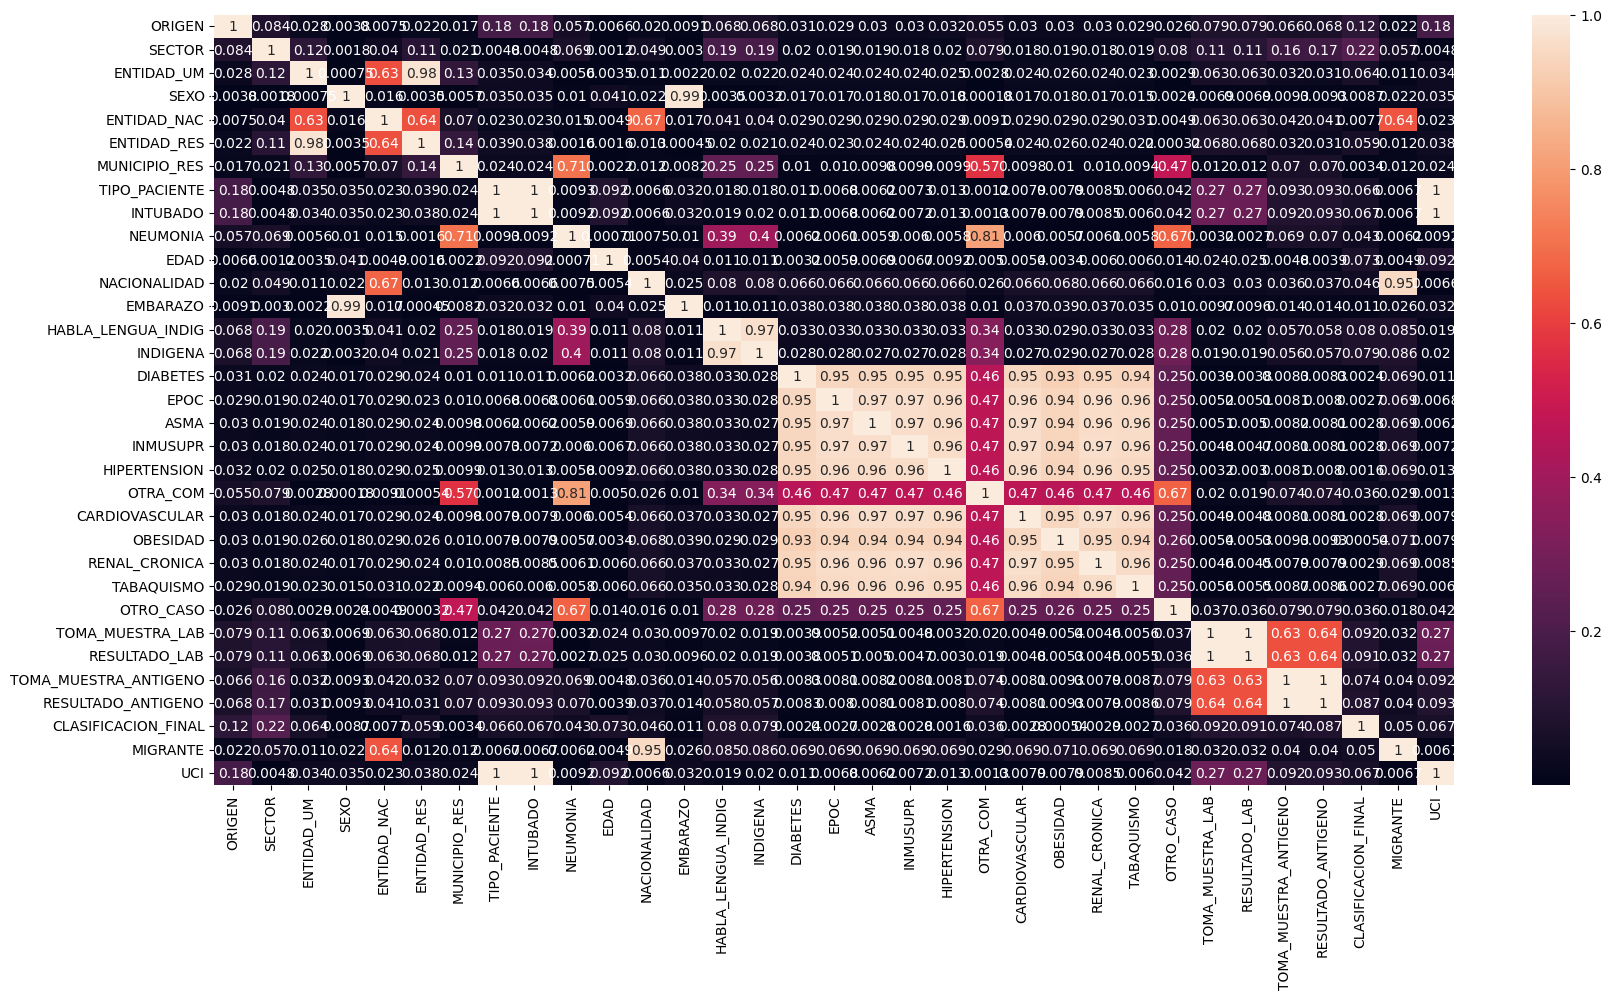
\includegraphics[scale=.4] {img/a-correlacion}
	\caption{Matriz de correlación}
	\label{fig:0}	
\end{figure}

% ------------------------------------------------------------------------------
% REFERENCIAS, revisar configuración \stylecitereferences
% ------------------------------------------------------------------------------
\clearpage
\bibliography{library} 